\documentclass[12pt]{article}
\usepackage{enumerate}
\usepackage{amsmath}
\usepackage{amssymb}
\usepackage{amsthm}
\usepackage{etoolbox}
\usepackage{graphicx}

\newcommand{\Name}[1]{\noindent \textbf{Name:} #1 \\}
\newcommand{\Workedwith}[1]{\noindent \textbf{Worked with:} #1 \\}
\newcommand{\Problem}[3]{\mbox{} \newline \noindent \textbf{\textbf{Problem #1: #2 [#3 Points] \\ }}}


\begin{document}

\begin{center}
  \bf
  Algorithms \\
  CMPT 307 D200 \\
  Spring 2024 \\
  \rm
  Homework 5\\
  Due:  Sunday, Mar 31 at 10:00 PM \\
\end{center}

\Name{Your name here}
\Workedwith{Everyone you worked with here}

\Problem{6}{Bonus Problem! Digital Circuits}{25}

(This problem is extra credit! The setup for the problem might seem intimidating and long, but this question is comparable in difficulty to the other problems on this assignment. If you have time, I highly recommend you give it a go!)

My day job is as a software engineer at a company called Altera (owned by Intel).
Altera makes digital devices called Field Programmable Gate Arrays (FPGAs), which, in short, simulate digital logic.
Here's a real-world problem that I've actually worked on at my company.

There are two main categories of digital logic: combinational and sequential.
Combinational logic (also known as time-independent logic) is logic whose output is solely a function of the present input.
Sequential logic, on the other hand, is logic whose output also depends on past inputs.

For example, if you have a circuit that you can give two numbers, one after the other, and then the circuit computes the addition of those two numbers, that would be sequential logic. On the other hand, if it took both numbers simultaneously, that could be implemented with only combinational logic.

Sequential logic is much more powerful (and, for example, CPUs inherently need sequential logic to operate), but also much harder to reason about. As a result, a good rule of thumb in digital design is to try to contain the sequential parts to particular parts of your circuit design. Generally, this is done by having circuits called ``registers'' in your design, and everything else uses solely combinational logic.

The main building blocks of combinational logic are logic gates you're probably familiar with - AND, OR, NOT, etc.
Note also that combinational logic never has cycles - outputs strictly ``feed forwards''.

The main building block of sequential logic is a device called a register. A register has one main input ($D$) and one main output ($Q$). It also accepts a clock signal, which is generally a signal that starts at 0 and then flips to 1 after some amount of time, then flips back to 0 after the same amount of time, and continues on infinitely.
On the rising edge of the clock (that is, when the clock goes from 0 to 1), the register sets its output $Q$ to the value it sees at its input $D$.
If $D$ changes after this point, the register still holds the old value it saw
(Note: this is a bit of a simplification for the sake of this problem. I don't want to get into details about registers beyond what I've already said... Digital electronics is a fractally nested set of abstractions; there is no bottom.)

So basically, most digital circuits comprise a bunch of registers, with combinational logic between them.

When considering the group of combinational logic that feeds into a particular register, you can walk backwards through the circuit until you hit a register. All of the nodes you can reach traveling backwards without passing through a register are important to consider.

Each gate in a combinational circuit has two types of delays: propagation delay ($t_{pd}$) and contamination delay ($t_{cd}$).
Propagation delay is how long it takes for the output to be the right answer after the input changes, and contamination delay is how long it takes for the output to become invalid once a new input is given.
So you shouldn't trust the signal coming out of a particular gate until $t_{pd}$ after the input changes.
On the other hand, when the input changes, you still have $t_{cd}$ time before the output becomes invalid.
Note that $t_{pd} \geq t_{cd}$.

The gist of contamination delay is that it corresponds to the soonest the output might change, and it might change to some intermediate state that is not yet valid.
The gist of propagation delay is that it corresponds to how long you might have to wait before the value is definitely correct.

For example, let's consider an XOR gate. This gate has two inputs (let's call them $A$ and $B$) and one output ($C$), and the output is 1 if and only if exactly one of the inputs has value 1.
Currently, this gate has exactly one of its inputs as 1 (let's say $A = 1; B = 0$), so its output is 1.
If we toggle both of its inputs simultaneously (so now $A = 0; B = 1$), its output should still be 1.
However, due to complexities with how the XOR gate works, its output actually switches to zero before it switches back to 1.
Let's say you switched the inputs at time $t$.
You can trust that the output still has the old answer (1) until at least $t + t_{cd}$, and you can trust that the output has the correct new answer any time after $t + t_{pd}$.

Wires between gates also have some delay, and this delay is added to both the contamination and propagation delays when considering overall propagation and contamination delays.
In a combinational circuit, the overall contamination delay is given by the sum of contamination delays (plus the delays from wires) along the \textit{shortest} path through the circuit.
On the other hand, the overall propagation delay is given by the sum of propagation delays (plus the delays from wires) along the \textit{longest} path through the circuit.

Here's a concrete example.
Let's say we want to determine the contamination and propagation delays for the combinational circuit that feeds into a particular register.
Here's the schematic:

\begin{centering}
  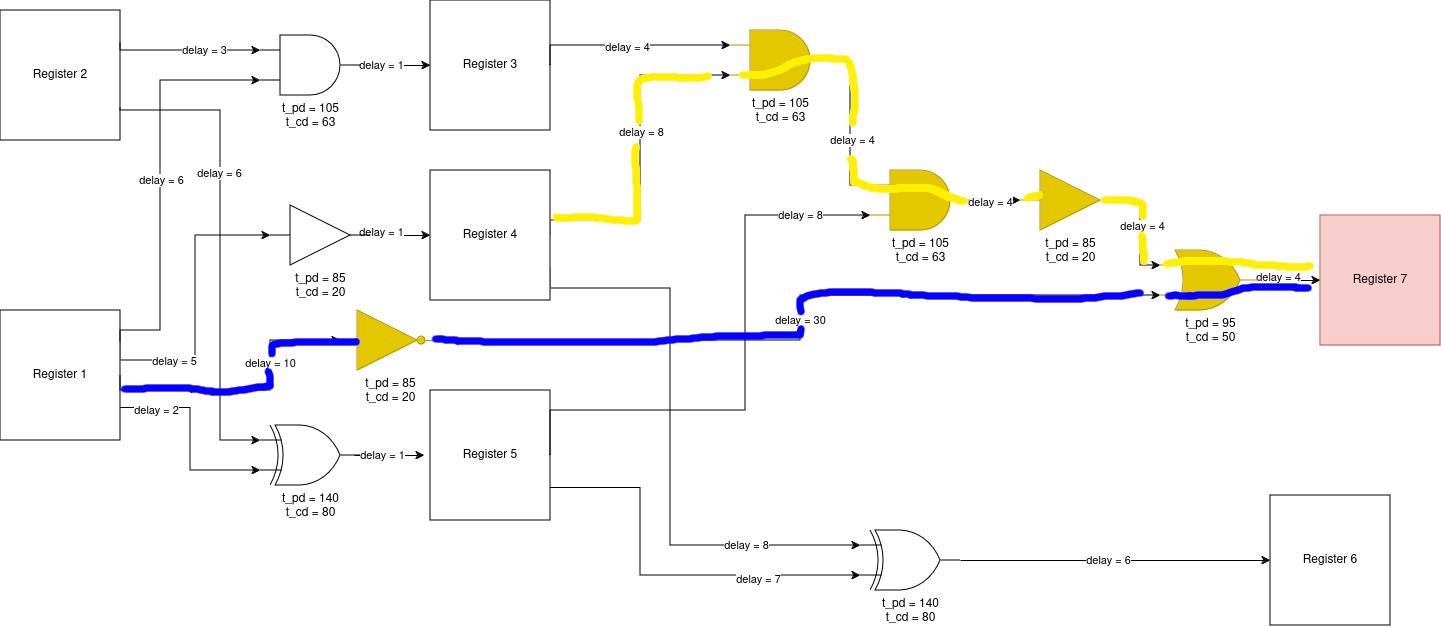
\includegraphics[width=\linewidth]{schematic}
\end{centering}


In this diagram, inputs are on the left side of nodes and outputs are on the right side. If a register has two or more outputs, they are the same signal. You can assume that each wire corresponds to an edge.
The register highlighted in red (register 7) is the one we care about.
The 5 gates highlighted in gold are the combinational logic that feeds into the red register, so they're the only parts of the circuit we have to consider.
The shortest path through that combinational logic, starting at any previous register, is highlighted in blue.
The longest path through that combinational logic, starting at any previous register, is highlighted in yellow.

Thus, the total propagation delay for the logic feeding into this register is the sum along the blue path, which is $(10 + 20 + 30 + 50 + 4) = 114$.
The total contamination delay for the logic feeding into this register is the sum along the yellow path, which is $(8 + 105 + 4 + 105 + 4 + 85 + 4 + 95 + 4) = 414$.

Given a circuit and a particular register, compute the contamination and propagation delays for the combinational logic that feeds into this register.
You may assume that the circuit is specified as a directed weighted graph $G = (V, E)$ with $m = |E|$ and $n = |V|$.
The weights on the edges in the graph correspond to the delays through the wires.

Each node is either a gate or a register.
There is a function $\textsc{IsRegister}(u)$ that returns either \textsc{True} or \textsc{False}, representing whether or not a particular node $u$ is a register.
There are also functions $\textsc{GetPropagationDelay}(v)$ and $\textsc{GetContaminationDelay}(v)$ that will return the propagation delay and contamination delay, respectively, of a particular non-register node $v$.
You can assume that the specified register will always have inputs.

You should solve this in 4 steps:
\begin{enumerate}
  \item Figure out which nodes are relevant for determining the contamination and propagation delays. (You can modify an algorithm we've already seen for this step.)
  \item Build 2 graphs, one for contamination and one for propagation.
  \item Use these graphs and off-the-shelf shortest path graph algorithms to compute the propagation and contamination delays. You should not have to modify the algorithm you end up using; if needed, modify your graph from part (2) instead.
  \item Compute the runtime of all of these steps.
\end{enumerate}

(If you're interested in this, and also interested in digital logic, I encourage you to take a class like ENSC 252! If you don't have the bandwidth to take that class but want to read more about this subject matter, \textit{Digital Design and Computer Architecture: ARM Edition} by David Harris and Sarah Harris is the authoritative book on computer engineering and digital logic.)


\textbf{Solution:}

Your solution goes here.

\bigbreak
\bigbreak
\bigbreak
\bigbreak
\bigbreak

\textbf{Bonus Info about the Problem}

This section is not necessary to read, but helps motivate the problem a little more.
The longest propagation delay of any combinational logic between two registers affects the maximum clock speed at which you can run your design.
Think CPU clock frequency, e.g. 4GHz.

Contamination delay comes up because registers are imperfect and their values don't change immediately, and the value at the input has to be present for some amount of time before the register will accept it.
They're also only guaranteed to hold the correct signal for a certain amount of time.
So this also affects how fast you can run your design.
Well-designed circuits are optimized to keep propagation and contamination delays for a given block of combinational logic similar, since then neither will be the limiting factor for increasing the clock speed of the design.

So if you are designing digital logic, you want to be able to easily find critical timing paths for both contamination and propagation delay.
The task that I've been working on for the last month or two at work involves writing code that visualizes these critical timing paths so that users can more easily optimize their design in order to remove bottlenecks on max clock frequency.



\end{document}
